\section{Auswertung und Diskussion}
\label{sec:Auswertung}

In den Abbildungen \ref{abb:Z}, \ref{abb:Y} und \ref{abb:X} ist die resultierende
Dosisverteilung aus verschiedenen Ansichten dargestellt.
Dabei ist das PTV in rot dargestellt und die Isodosenlinien in den angegebenen Farben.
Anhand der Dosisverteilungen ist zu erkennen, dass ein Großteil des PTVs mit der $95\%$ Isodosenlinie
umschlossen werden konnte. In Abbildung \ref{abb:X}, in der sagittalen Ansicht, ist allerdings
zu erkennen, dass im unteren Bereich des PTVs eine relative Dosis von $95\%$ nicht erreicht werden konnte.
Das liegt daran, dass sich in diesem Bereich viel Gewebe und Knochen in dem Strahlengang befinden und
somit dort die Dosis stärker abgeschwächt wird.
Aus diesem Grund ist die minimale relative Dosis im PTV $82,6\%$ und liegt unterhalb der gewünschten relativen Dosis von $95\%$.
Außerdem fällt auf, dass die maximale relative Dosis $113,3\%$ außerhalb des PTVs deponiert wird. Anhand der Darstellungen
der Dosisverteilungen ist zu erkennen, dass die maximale Dosis in dem Schädelknochen deponiert wird. Das ist zu erwarten gewesen, da
der Schädelknochen, durch seine hohe Dichte, viel Dosis absorbiert. Da das gesamte PTV von dem Schädelknochen umgeben ist, muss bereits
in dem Schädelknochen eine hohe Dosis deponiert werden damit in dem PTV noch die gewünschte Dosis ankommt.
In dem PTV wird eine maximale relative Dosis von $110\%$ deponiert. Diese maximale Dosis liegt auch über dem erlaubten Wert von $107\%$ \cite{ICRU}.
Anhand der Dosisverteilung ist aber zu erkennen, dass nur ein sehr geringer Teil des Großhirns eine so hohe Dosis erhält.

\begin{figure}[H]
  \centering
  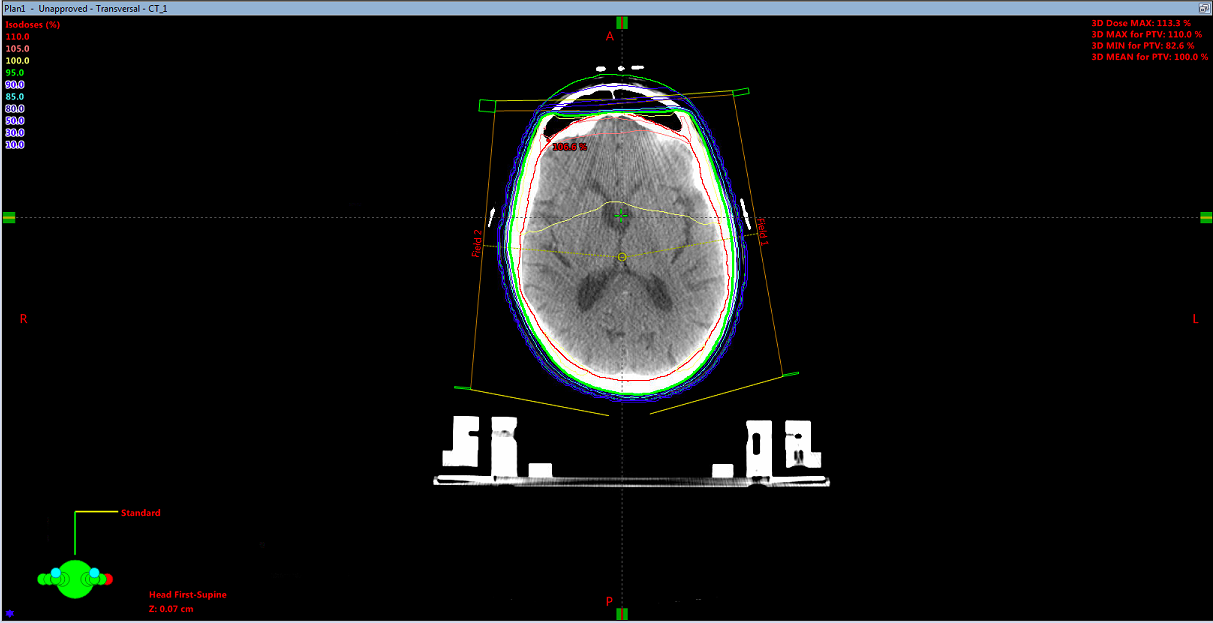
\includegraphics[width=\textwidth]{Bilder/Hirn_z.png}
  \caption{Darstellung der Dosisverteilung im Kopf in Transversalansicht.}
  \label{abb:Z}
\end{figure}

\begin{figure}[H]
  \centering
  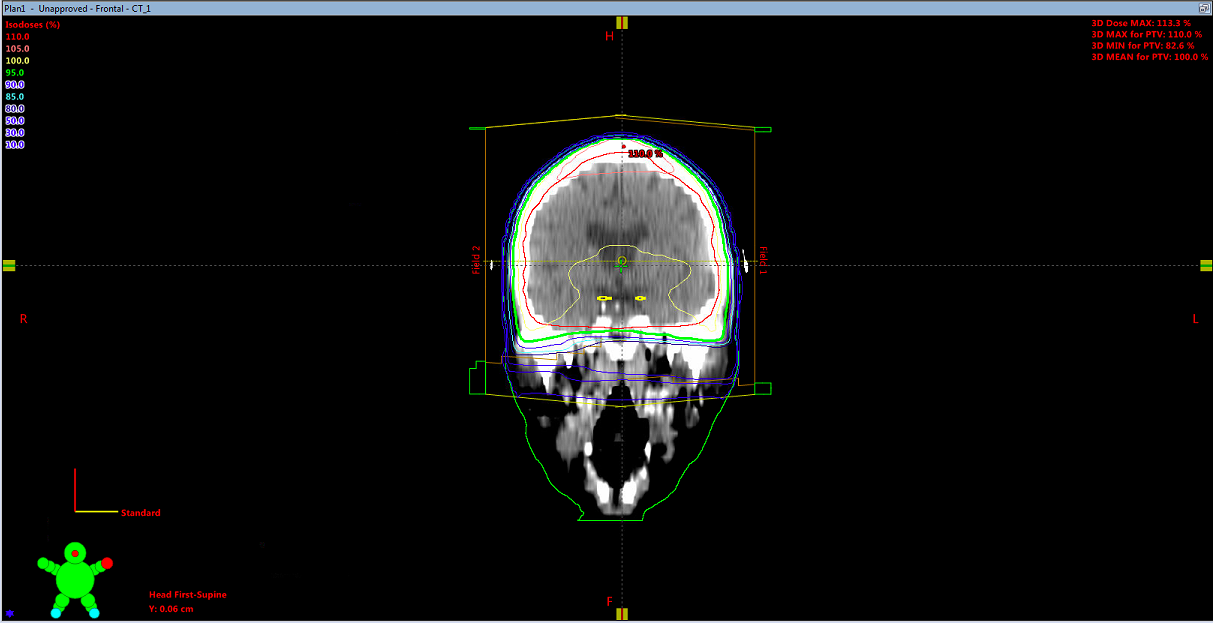
\includegraphics[width=\textwidth]{Bilder/Hirn_y.png}
  \caption{Darstellung der Dosisverteilung im Kopf in Frontalansicht.}
  \label{abb:Y}
\end{figure}

\begin{figure}[H]
  \centering
  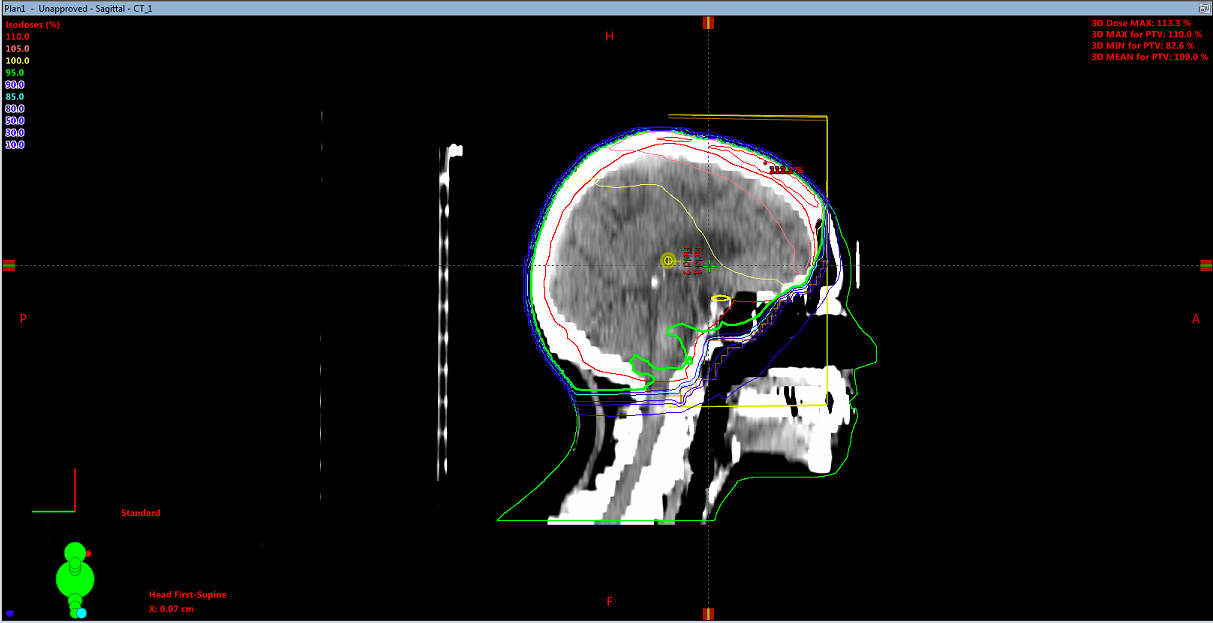
\includegraphics[width=\textwidth]{Bilder/Hirn_x.png}
  \caption{Darstellung der Dosisverteilung im Kopf in Sagittalansicht.}
  \label{abb:X}
\end{figure}

In der Abbildung \ref{abb:DVH} ist das zugehörige DVH dargestellt. Dabei ist zum einen das DVH des PTVs und des gesamten Schädels dargestellt und zum
anderen die Risikoorgane.
Anhand der Kurve für das PTV, in rot dargestellt, ist zu erkennen, dass nur ein sehr kleiner prozentualer Anteil des PTVs eine geringere relative Dosis als
$95\%$ erhält. Etwa $98\%$ des PTVs erhält noch eine relative Dosis von $95\%$.
Außerdem ist, wie bereits erwähnt, zu sehen, dass nur ein sehr geringer Teil von etwa $1-2\%$ des PTVs eine Dosis von mehr als $107\%$ erhält.
Das ist auch anhand der grünen Kurve für den gesamten Schädel zu erkennen. Der Teil des gesamten Schädels, der eine Dosis von über $107\%$ erhält ist
auch sehr gering. Es ist außerdem zu erkennen, dass der gesamte Schädel relativ viel Dosis erhält. Das kommt daher, da das PTV bei dieser Bestrahlung sehr
groß ist. Noch etwa $60\%$ des gesamten Schädels erhält $50\%$ der relativen Dosis.


\begin{figure}[H]
  \centering
  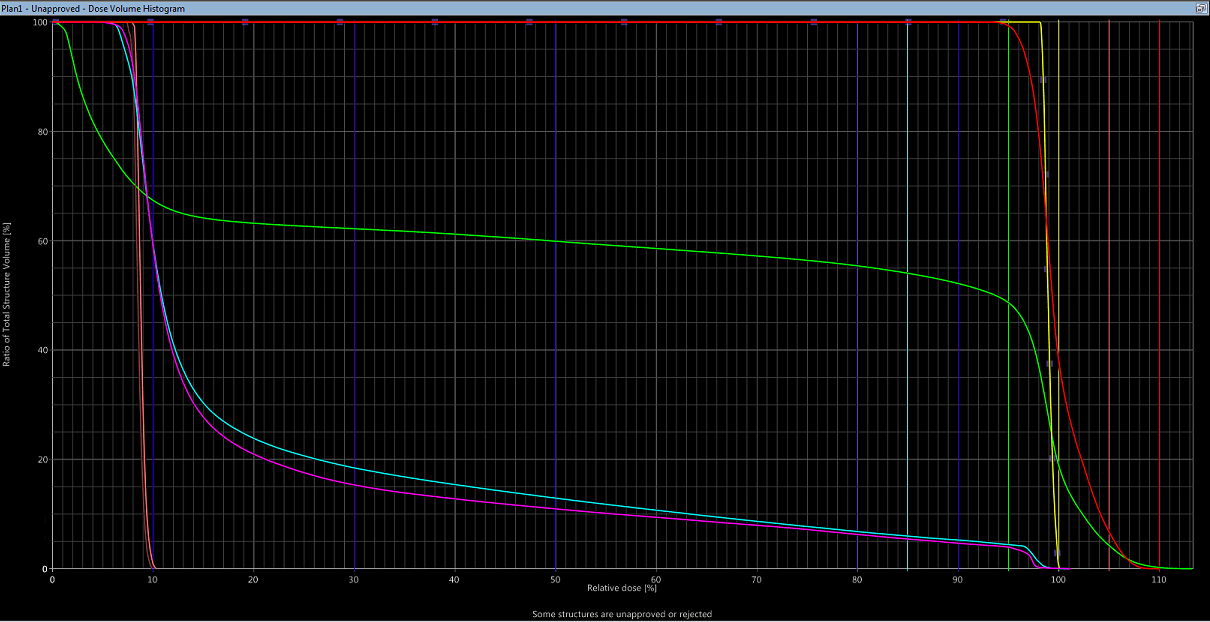
\includegraphics[width=\textwidth]{Bilder/Hirn_DVH.png}
  \caption{Dosis-Volumen-Histogramm für das PTV in rot und den gesamten Schädel in grün. Außerdem ist das DVH für das Chiasma in gelb, für die linke Linse in pink, für die rechte Linse in braun, für das linke Auge in lila und für das rechte Auge in hellblau dargestellt.}
  \label{abb:DVH}
\end{figure}

Da bei dieser Strahlentherapie mit einer hohen Dosis bestrahlt wird, müssen die Dosisgrenzwerte für
die Risikoorgane beachtet werden. Die maximale Dosis der Augenlinsen darf $\SI{5}{\gray}$ nicht überschreiten \cite{grenz}.
In diesem Bestrahlungsplan ist die maximale Dosis der Linsen $10\%$ und $10,3\%$. Da mit einer Gesamtdosis von $\SI{45}{\gray}$ bestrahlt werden
soll ergibt sich eine maximale Dosis für die Augenlinsen von $\SI{4.5}{\gray}$ und $\SI{4.6}{\gray}$. Diese maximale Dosen liegen unterhalb des Grenzwertes.
Anhand der DVHs der gesamten Augen ist zu erkennen, dass etwa $20\%$ (bzw. $25\%$) der Augen eine relative Dosis von $20\%$ erhalten und nur noch etwa
$10\%$ (bzw. $12\%$) eine Dosis von $50\%$. Ein weiteres Risikoorgan ist das Chiasma Opticum. Die maximale Dosis des Chiasmas beträgt $\SI{54}{\gray}$
\cite{grenz}. Die maximale relative Dosis des Chiasmas in diesem Plan beträgt $100,1\%$ und somit etwa $\SI{45}{\gray}$. Somit wird auch der Grenzwert
für das Chiasma Opticum nicht überschritten. \\

Durch Verwendung von zwei Feldern, welche seitlich auf den Kopf treffen, ist es möglich
die gewünschte Dosisverteilung weitgehend zu erreichen. Bis auf einen sehr kleinen Teil ist
es gelungen, dass das PTV mit der $95\%$ Isodosenlinie umschlossen wird. Außerdem ist es durch die
verwendeten MLCs gelungen, dass der Organdosisgrenzwert der Augenlinsen nicht überschritten wird.
